\documentclass[12pt,a4paper]{article}
\usepackage[utf8]{inputenc}
\usepackage{amsmath}
\usepackage[brazilian]{babel} % Brazil or not Brazil??
\usepackage{amsfonts}
\usepackage{amssymb}
\usepackage{graphicx}
\usepackage[margin=0.8in]{geometry}


\begin{document}
\title{\vspace{70mm}\Huge Experimento 06a - Calorimetria}
\author{ Giovani Garuffi\qquad\hfill
		\textit {RA: 155559}\protect\\
		João Baraldi\hfill
		\textit{RA: 158044}\protect\\
		Lauro Cruz\hfill
		\textit{RA: 156175}\protect\\
		Lucas Schanner\hfill
		\textit{RA: 156412}\protect\\
		Pedro Stringhini\hfill
		\textit {RA: 156983}								
		}
\maketitle
\newpage
\section{Resumo}

\section{Objetivos}
Este experimento pode ser divido em duas partes, cada uma com seus objetivos, que são: a determinação do calor específico de três metais diferentes (acreditados de serem chumbo, alumínio e cobre), e a determinação do calor latente de fusão do gelo. 


\section{Procedimento Experimental e Coleta de Dados}


\subsection{Procedimento}


\subsubsection{Determinação do Calor Específico de Metais}

%acentuar palavras 

Esta parte do experimento foi feita da seguinte maneira: com um ebulidor, aquece-se uma amostra de áagua, numa garrafa térmica, e imerge-se a amostra do metal, de massa obtida com uma balança, nessa água, mantendo-se o controle de sua temperatura com um termômetro de mercúrio. Então, insere-se o metal aquecido no calorímetro com água fria (vide figura \ref{CalorMetais}), de temperatura e massa também conhecidas, e espera-se pelo equílibrio térmico registrando o valor da temperatura nesse estado.

\begin{figure}[!htbp]
\centering
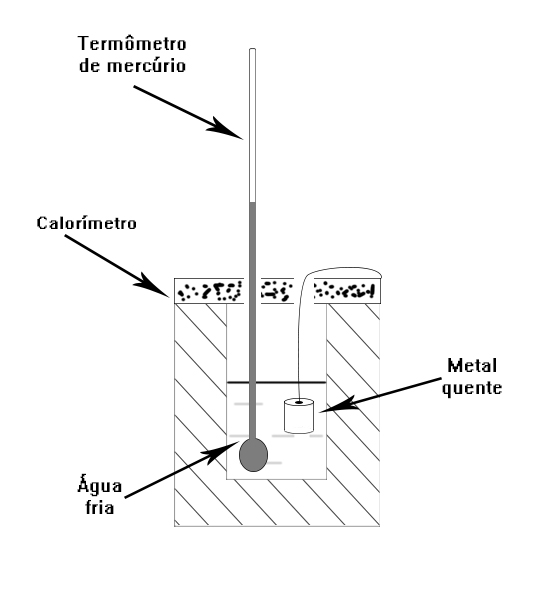
\includegraphics[scale=0.55]{Fig6b1.jpg}
\caption{Exemplo da montagem experimental da primeira parte do experimento.}
\label{CalorMetais}
\end{figure}

Ent~ao, repete-se o procedimento para as demais amostras.

\subsubsection{Determinação do Calor Latente de Fusão do Gelo}

Esta outra parte é feita de forma análoga à anterior. Insere-se uma massa $m$ (encontrado com a balança) de gelo, de temperatura conhecida, no calorímetro preenchido até a metade com agua fria, de massa e temperatura conhcidos, até atingir-se o equilíbrio térmico, medindo-se seu valor com o termômetro, como mostrado na figura \ref{CalorGelo}.

\begin{figure}[!htbp]
\centering
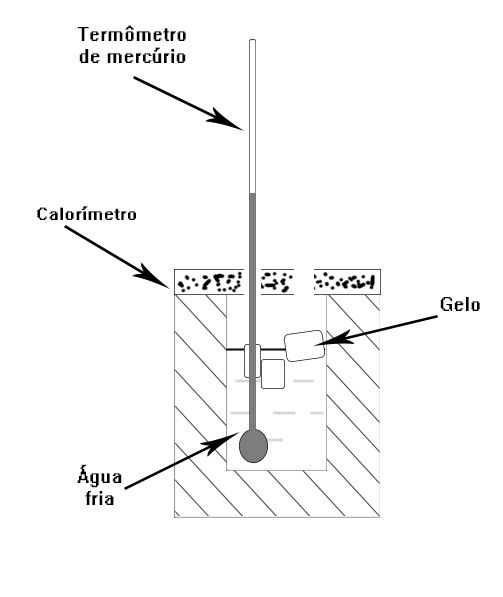
\includegraphics[scale=0.55]{Fig6b2.jpg}
\caption{Exemplo de montagem experimental da segunda parte do experimento.}
\label{CalorGelo}
\end{figure}


\section{Análise dos Resultados e Discussões}


\subsection{Determinação do Calor Específico de Metais}

%ficou feio esse primeiro paragrafo não-identado... Se quiser mudar tem uma \usepackage{indentfirst} que é sucesso.
Para o chumbo, obtivemos os seguintes valores:
$$ T_{quente} = (75,0 \pm 0,5)\,^{\circ}\mathrm{C}, \qquad T_{frio} = (22,0 \pm 0,5)\,^{\circ}\mathrm{C}, $$
$$ T_{Metal} = (102,0 \pm 0,5)\,^{\circ}\mathrm{C}, \qquad T_{equilibrio} = (23,0 \pm 0,5)\,^{\circ}\mathrm{C}. $$


Para o alumínio, obtivemos os seguintes valores:
$$ T_{quente} = (72,5 \pm 0,5)\,^{\circ}\mathrm{C}, \qquad T_{frio} = (24,0 \pm 0,5)\,^{\circ}\mathrm{C}, $$
$$ T_{Metal} = (42,3 \pm 0,1)\,^{\circ}\mathrm{C}, \qquad T_{equilibrio} = (26,0 \pm 0,5)\,^{\circ}\mathrm{C}. $$


 E finalmente, para o cobre, temos:
$$ T_{quente} = (67,0 \pm 0,5)\,^{\circ}\mathrm{C}, \qquad T_{frio} = (26,5 \pm 0,5)\,^{\circ}\mathrm{C}, $$
$$ T_{Metal} = (91,6 \pm 0,1)\,^{\circ}\mathrm{C}, \qquad T_{equilibrio} = (27,5 \pm 0,5)\,^{\circ}\mathrm{C}. $$

Sabendo que a massa de água fria utilizada foi de $(185 \pm 0,5)g$, tem-se que os calores específicos dos metais são:

\subsection{Determinação do Calor Latente de Fusão do Gelo}


\section{Conclusões}

\end{document}

